\newpage
\section{Dashboard \& Additional Features Overview}
The University Management System (UMS) contains a dashboard as shown in \autoref{fig:example3} and initial features upon logging in with the correct credentials. First, the additional features once a user logs in are the collapse menu button and the logout button. Both of these buttons are consistent across all types of users (e.g., student, faculty of administrators). The collapse menu allows the user to hide the navigation panel or keep it open, and the logout button once clicked places the user back into the login page at the start of the program. In the upper right corner, the UMS has the feature to maximize, minimize, and close the software. Each of these buttons is designed to ensure that the software integration remains seamless once pressed.


The UMS also contains a viewable dashboard after logging in, providing key statistics and relevant numbers for quick understanding. The dashboard, as shown in \autoref{fig:example3}, is the initial page that provides an overview. Provides an overview of all students, courses, faculty, and events within the University.


\begin{figure}[ht]
    \centering
        \centering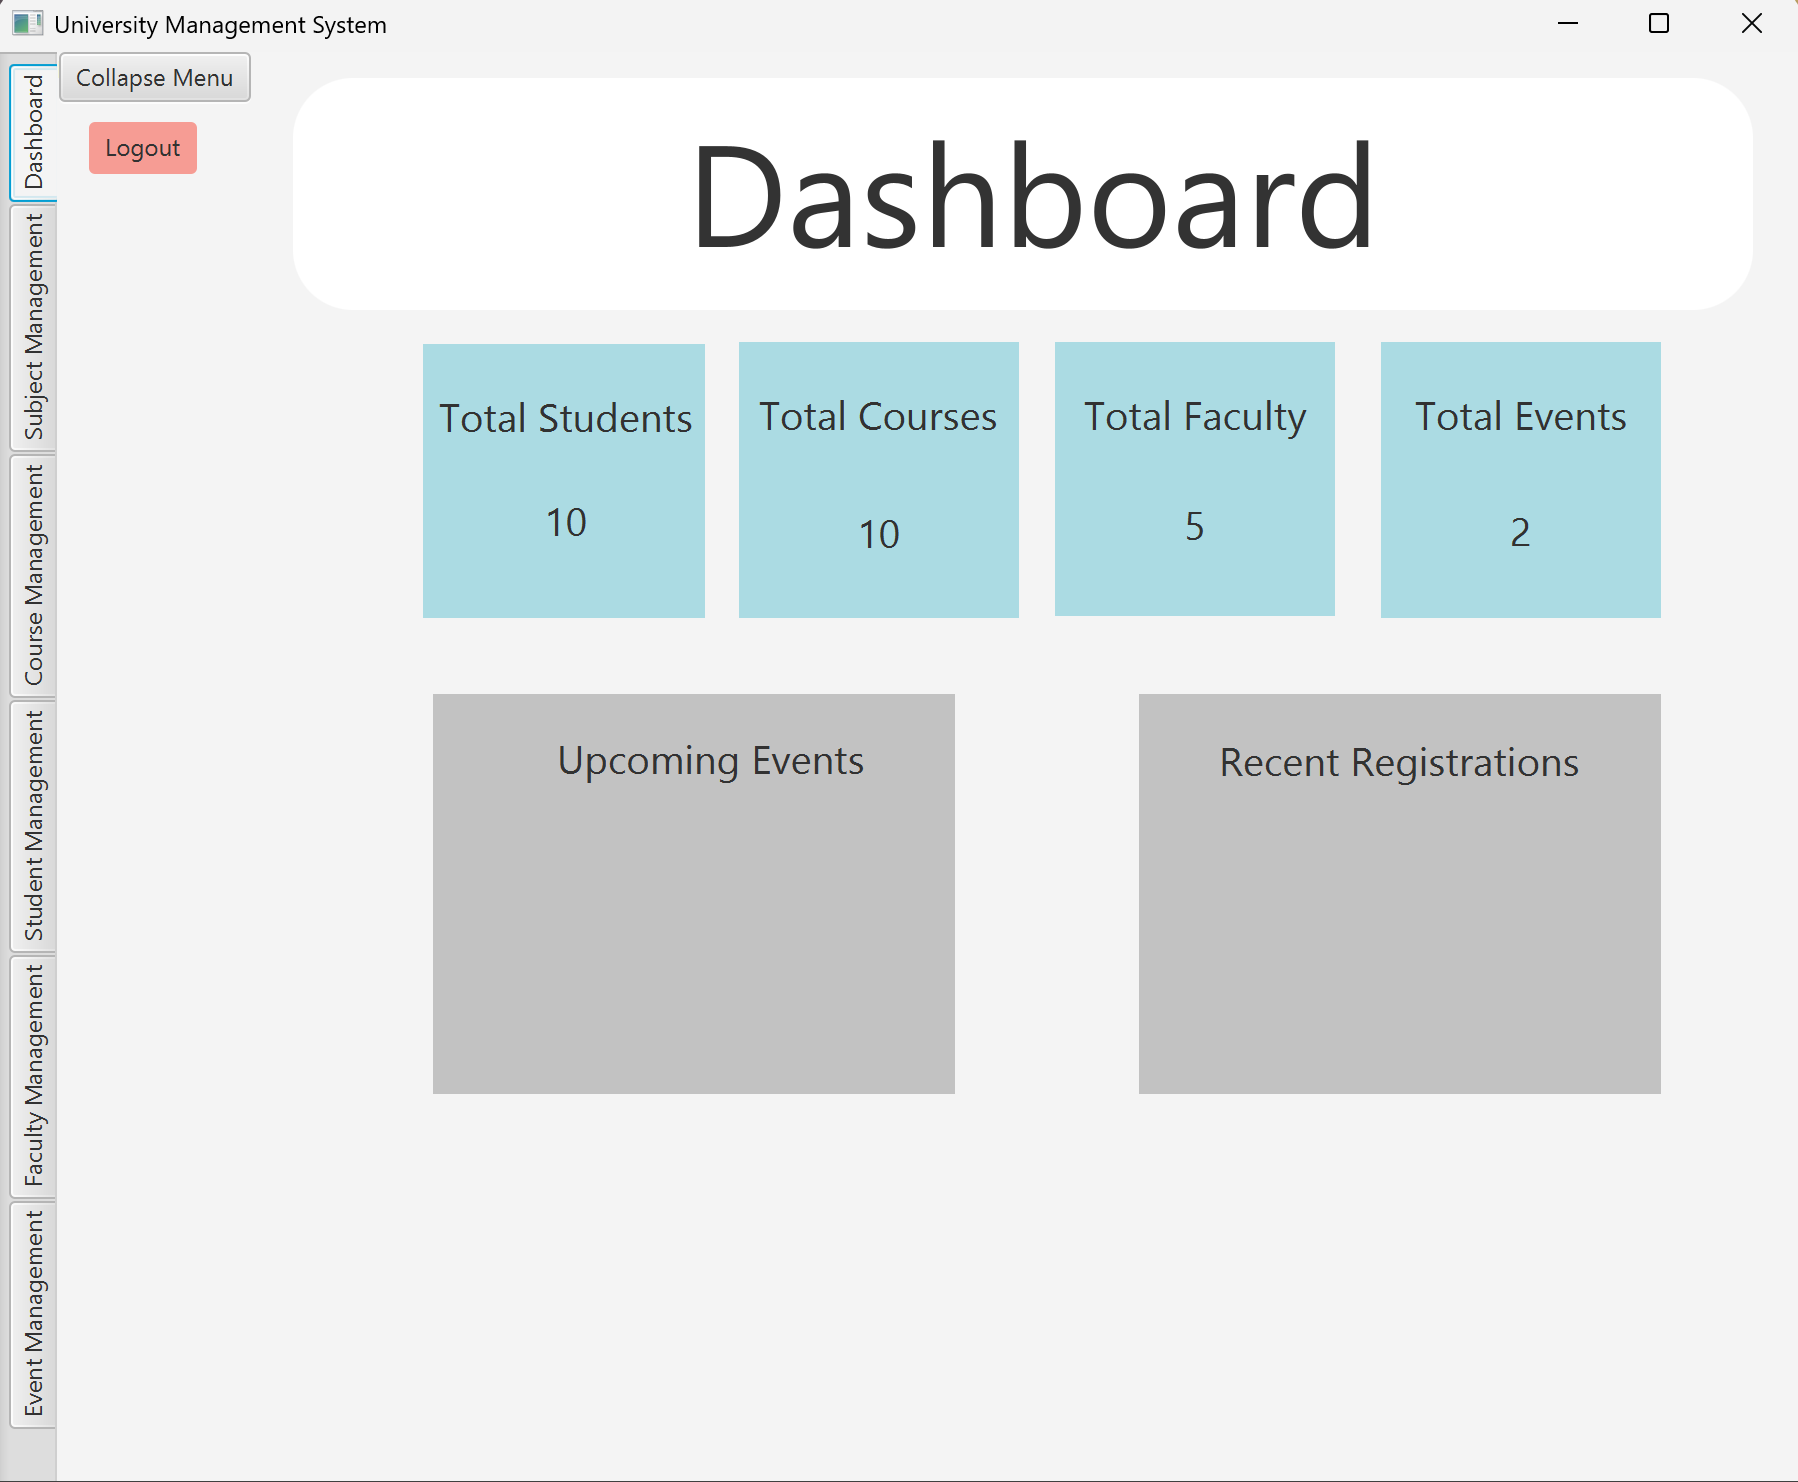
\includegraphics[width=0.7\linewidth]{figures/Dashboard.png}
        \caption{Dashboard}
        \label{fig:example3}  
\end{figure}



\newpage
\subsection{Navigation Menu}
The University Management System (UMS) contains a navigation panel on the left side of the program once the correct user logins. These have the following tabs; Dashboard, Subject Management, Course Management, Student Management, Faculty Management, and Event Management, as shown in \autoref{fig:example4}. Each of these tabs are clickable, allowing the user to move throughout each one. More details on each page are provided in subsequent sections. 

\begin{itemize}
    \item Subject Management: Overview of Subjects at the University.
    \item Course Management: Overview of all the courses, subject code, capacity, lecture time, exam, location and teacher offered at the University.
    \item Student Management: Overview of the Student at the University.
    \item Faculty Management: Overview of the Faculty at the University.
    \item Event Management: Schedule of all the events at the University.
\end{itemize}

\begin{figure}[h!]
    \centering
    \adjustbox{max width=0.125\linewidth}{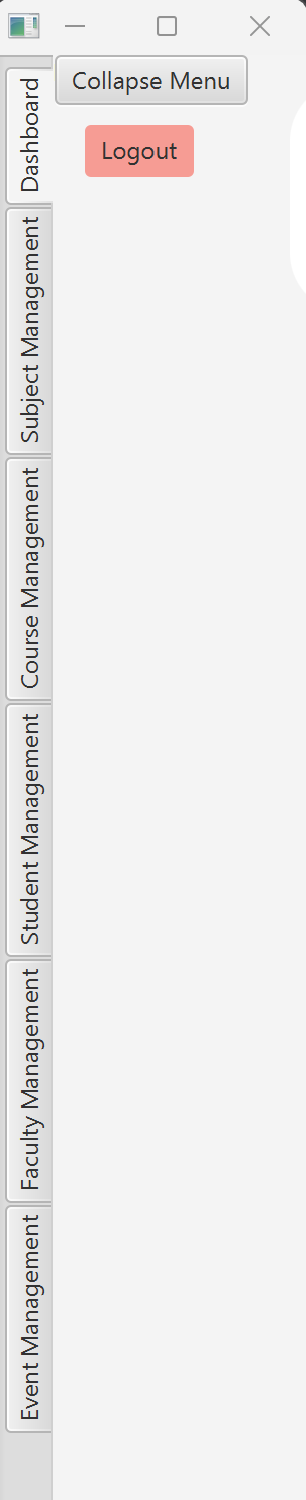
\includegraphics{figures/Navigation_Menu.png}}
    \caption{Navigation Panel}
    \label{fig:example4}
\end{figure}
\FloatBarrier


% \begin{figure}[h!]
%     \centering
%     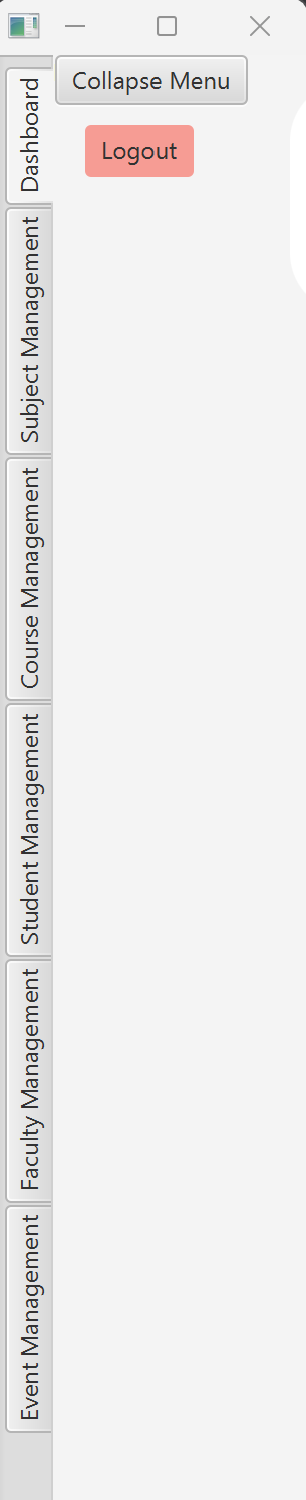
\includegraphics[width=0.45\textwidth]{figures/Navigation_Menu.png}
%     \caption{Dashboard}
% \end{figure}
% \FloatBarrier